\documentclass[journal]{IEEEtran}
\usepackage[T1]{fontenc}
\usepackage{graphicx}
\usepackage{booktabs}
\usepackage{amsmath}
\usepackage[hidelinks]{hyperref}
\title{Coordinate Auxiliary Supervision for Spatial Hangul Jamo Generation: An Exploratory Ablation Study}
\author{Jisu Kang\thanks{Jisu Kang is with the AIFFEL Research Course, Cohort 19. This manuscript reports a course research project and has not been published in an IEEE journal.}}
\begin{document}
\maketitle
\begin{abstract}
Spatially separated Hangul jamo require a generator to preserve both letter identity and two-dimensional placement within a linear text output. This study examines whether coordinate auxiliary supervision improves a small decoder-only model on a fixed Korean-to-jamo formatting task. We construct 248 synthetic examples, split into 198 training, 25 validation, and 25 test items, and compare unadapted Qwen2.5-0.5B-Instruct with three LoRA conditions: conversion only, conversion with character-list supervision, and conversion with character-coordinate supervision. The trained conditions are initialized independently from the same backbone and evaluated at fixed epochs five and ten. At epoch ten, character-coordinate micro F1 is 26.36\%, 22.16\%, and 28.41\%, respectively. Coordinate supervision exceeds character-list supervision by 6.25 percentage points on this diagnostic, but both obtain 0/25 exact layouts; conversion-only training obtains 1/25. All three conditions improve their partial scores from five to ten epochs. A separate OCR pilot fails to preserve complete character inventories in ten images, so the training labels are synthetic rather than OCR-derived. These exploratory results suggest a limited advantage in partial spatial matching, without demonstrating improved complete generation. Single-seed training, a reused test set, small sample size, and unequal auxiliary token budgets constrain interpretation.
\end{abstract}
\begin{IEEEkeywords}
Hangul jamo, spatial text generation, auxiliary supervision, parameter-efficient fine-tuning, layout evaluation.
\end{IEEEkeywords}

\section{Introduction}
\IEEEPARstart{H}{angul} represents Korean syllables using consonant and vowel letters called jamo. A syllable normally combines an initial consonant, a vowel, and optionally a final consonant in a compact block. Korean users can deliberately separate these letters with spaces and newlines to create a spatial writing style. A generator must then recover the required letters and place each one correctly; an appropriate set of letters alone does not guarantee a valid layout.

The motivating observation arose during an interaction with a commercial language-model service: it appeared to interpret a spatial jamo example but did not reliably reproduce the requested layout for another input. This is an anecdotal motivation, not a quantified reading--writing comparison. We do not evaluate that service or measure semantic comprehension. Instead, we define a narrow, reproducible task: convert ordinary Korean text into one explicitly specified jamo grid.

Progress in Korean reasoning models, exemplified by HyperCLOVA X THINK~\cite{naver2025think}, does not directly answer this formatting question. Work on jamo-level input perturbations~\cite{lee2026jamo} and Korean text-rich visual understanding~\cite{hwang2025kreta} likewise motivates attention to Korean orthographic and visual structure, while addressing different outputs. Layout-aware document modeling~\cite{lu2025bounding} suggests a testable idea: explicit positions may help a decoder learn where characters belong. We examine this idea using synthetic character-coordinate targets during training, without supplying coordinates at inference.

The main research question is: \emph{Does character-coordinate auxiliary supervision improve exact spatial jamo generation beyond character-list supervision under a fixed small-data training configuration?} Secondary questions concern conversion-only fine-tuning and the effect of increasing training from five to ten epochs. We report a negative result on complete generation together with a positive but limited observation on partial spatial matching. The contributions are a fixed task definition and synthetic benchmark, a component comparison with distinct identity and position metrics, and an auditable analysis of failures across training, validation, and test inputs. The study does not establish a reliable converter or broad improvement in Korean language understanding.

\section{Related Work and Hypothesis Rationale}
\subsection{Korean capability and orthographic specificity}
HyperCLOVA X THINK combines Korean--English pretraining and post-training and evaluates Korea-centered reasoning and language tasks~\cite{naver2025think}. It supplies context for language-specific evaluation; its reported reasoning results are not evidence of success or failure on our jamo formatting task. Our inference is that fine-grained output requirements deserve direct measurement rather than being inferred from general Korean benchmark performance.

Lee and Lee investigate how jamo-level typographical perturbations affect language-model inputs~\cite{lee2026jamo}. Their distinction between syllable-level text and its internal letters motivates our separate assessment of character identity. However, their corrupted-input understanding task differs from intentional output decomposition. We extend the \emph{evaluation perspective} from input robustness to output construction, not their method or empirical findings. No claim that their measured vulnerability causes our errors is made.

\subsection{Reading, generation, and explicit layout}
KRETA evaluates Korean reading and reasoning in text-rich visual question answering across diverse visual contexts~\cite{hwang2025kreta}. Our task is complementary: the model must write a layout, rather than answer questions about a supplied image. This change in direction motivates position-sensitive generation evaluation. It does not make our benchmark an inverse of KRETA, nor establish that reading and writing share the same failure mechanism.

LayTextLLM projects bounding boxes into individual embeddings and interleaves them with text for document understanding~\cite{lu2025bounding}. This provides a rationale for testing explicit spatial information. Our implementation is materially different: a text-only decoder predicts serialized character--integer-coordinate entries as an auxiliary target. It has no bounding-box embedding module, image encoder, or OCR input at inference. Thus, the proposed transfer from layout-aware understanding to layout generation is a hypothesis to examine, not a consequence of the prior result.

\subsection{Research questions and operational hypotheses}
We distinguish complete task success from partial diagnostics. \textbf{H1 (adaptation)} expects conversion fine-tuning to improve task adherence relative to the unadapted backbone. \textbf{H2 (identity auxiliary task)} expects character-list supervision to help preserve the required character inventory relative to conversion-only training. \textbf{H3 (coordinate auxiliary task)} expects explicit coordinates to improve layout generation relative to character-list supervision. For H3, exact grid accuracy is the primary success criterion; character-coordinate F1 measures partial progress. More training is additionally examined through fixed epoch-five and epoch-ten comparisons.

These labels organize the research rationale; they are not a claim of prospective hypothesis preregistration. The coordinate question motivated the original experiment. The conversion-only control and partial-match diagnostics were introduced after inspecting its failures, and the extension protocol then fixed its conditions and checkpoints before the additional run. Consequently, the extension is exploratory even though its analysis settings were frozen in advance of that run.

\section{Task and Benchmark}
\subsection{Reference layout}
Let $x$ be ordinary Korean text and $G(x)$ its reference grid serialized using characters, ASCII spaces, and newlines. Every syllable's initial consonant occupies row zero. A vertical vowel occupies the cell immediately to its right, with the final consonant, if any, below the initial. A horizontal vowel occupies the cell below the initial, followed by the final consonant on the next row. Adjacent syllables have one empty separating cell; an original word space adds two more. Punctuation remains on row zero. Tense consonants and compound finals are each retained as one compatibility-jamo character. Each character or ASCII space occupies one grid cell, regardless of its font width.

\begin{figure}[t]
\centering

\includegraphics[width=.92\columnwidth]{figures/jamo_example.png}
\caption{Rule-generated reference for a three-syllable Korean name. Initial consonants share a top row. This is an annotation example, not a model prediction.}
\label{fig:reference}
\end{figure}

We exclude mixed-direction compound vowels and input newlines and permit only Korean text, ordinary spaces, and punctuation from the set \texttt{.,!?}. The input validator allows up to 24 characters. The benchmark itself covers shorter inputs, so this interface limit is not a tested capability. We do not model multiple styles, emoticons, general spam obfuscation, or ASCII logos. The reference converter could implement this fixed transformation without a neural model; the purpose is to study learned generation, not to demonstrate that a model is necessary.

\subsection{Data construction and separation}
A deterministic annotation program converts generic Korean words and short phrases into gold grids and character-coordinate lists. After scope filtering and exclusion of pilot phrases, 248 originals are split into 198 training, 25 validation, and 25 test items. Exact word-containment groups are kept within one split, although partial syllable and morpheme overlap remains. This evaluates new combinations in one known style, not unseen-letter or unseen-style generalization.

Training inputs span 1--10 characters, validation inputs 1--8, and test inputs 2--8, including spaces and punctuation. Multiword counts are 30, 5, and 4, respectively. Annotation checks include automatic consistency tests and representative visual inspection, not independent human review of every item. A fixed random subset of 12 training inputs is used for free-generation diagnosis; its results are not estimates of generalization or of accuracy across all 198 training items. Split files, identifiers, and hashes are retained.

\section{Method and Experimental Protocol}
\subsection{Backbone and component comparison}
We use Qwen2.5-0.5B-Instruct, a decoder-only instruction model, at revision \texttt{7ae5576}\footnote{Full revision: \texttt{7ae557604adf67be50417f59c2c2f167def9a775}. Model source: \url{https://huggingface.co/Qwen/Qwen2.5-0.5B-Instruct}.}. Table~\ref{tab:conditions} separates the unadapted baseline A from three fine-tuning conditions. D, B, and C are each restarted from the same backbone with the same seed. The extension does not resume the original five-epoch optimizer state, which was not retained.

\begin{table}[t]
\caption{Conditions and loss weights. All test-time inputs use the same conversion prompt; no gold coordinates or images are provided.}
\label{tab:conditions}\centering
\begin{tabular}{@{}clcc@{}}\toprule
 & Auxiliary target & Conversion & Auxiliary \\\midrule
A & No fine-tuning & -- & -- \\
D & None & 1.0 & 0.0 \\
B & Character list & 0.5 & 0.5 \\
C & Character-coordinate list & 0.5 & 0.5 \\\bottomrule
\end{tabular}
\end{table}

The main target is $G(x)$. Auxiliary entries follow left-to-right syllable order and initial--vowel--final order within each syllable. B predicts characters separated by semicolons. C predicts the identical character sequence augmented with zero-based grid coordinates in the form \texttt{character@x,y}. Coordinates are synthetic annotations. Both targets are learned through the same decoder with task-specific instructions; the conversion output does not pass through the auxiliary task at inference.

For B and C, the training objective is
\begin{equation}
\mathcal{L}=\tfrac12\mathcal{L}_{\mathrm{convert}}+\tfrac12\mathcal{L}_{\mathrm{aux}}.
\end{equation}
Each component is a mean next-token loss over its target tokens, including the end token; prompt tokens are masked. D uses only $\mathcal{L}_{\mathrm{convert}}$. The backbone weights are frozen and rank-8 LoRA adapters are applied to query and value projections, with alpha 16 and zero dropout. AdamW uses learning rate $2\times10^{-4}$ and weight decay 0.01. Gradients accumulate over eight originals, with norm clipping at 1.0. Ten epochs yield 250 optimizer updates per condition. Training uses float32 on a Tesla T4, seed 20260923, and a maximum sequence length of 1,536; overlength examples cause an error rather than silent truncation.

\begin{figure*}[t]
\centering
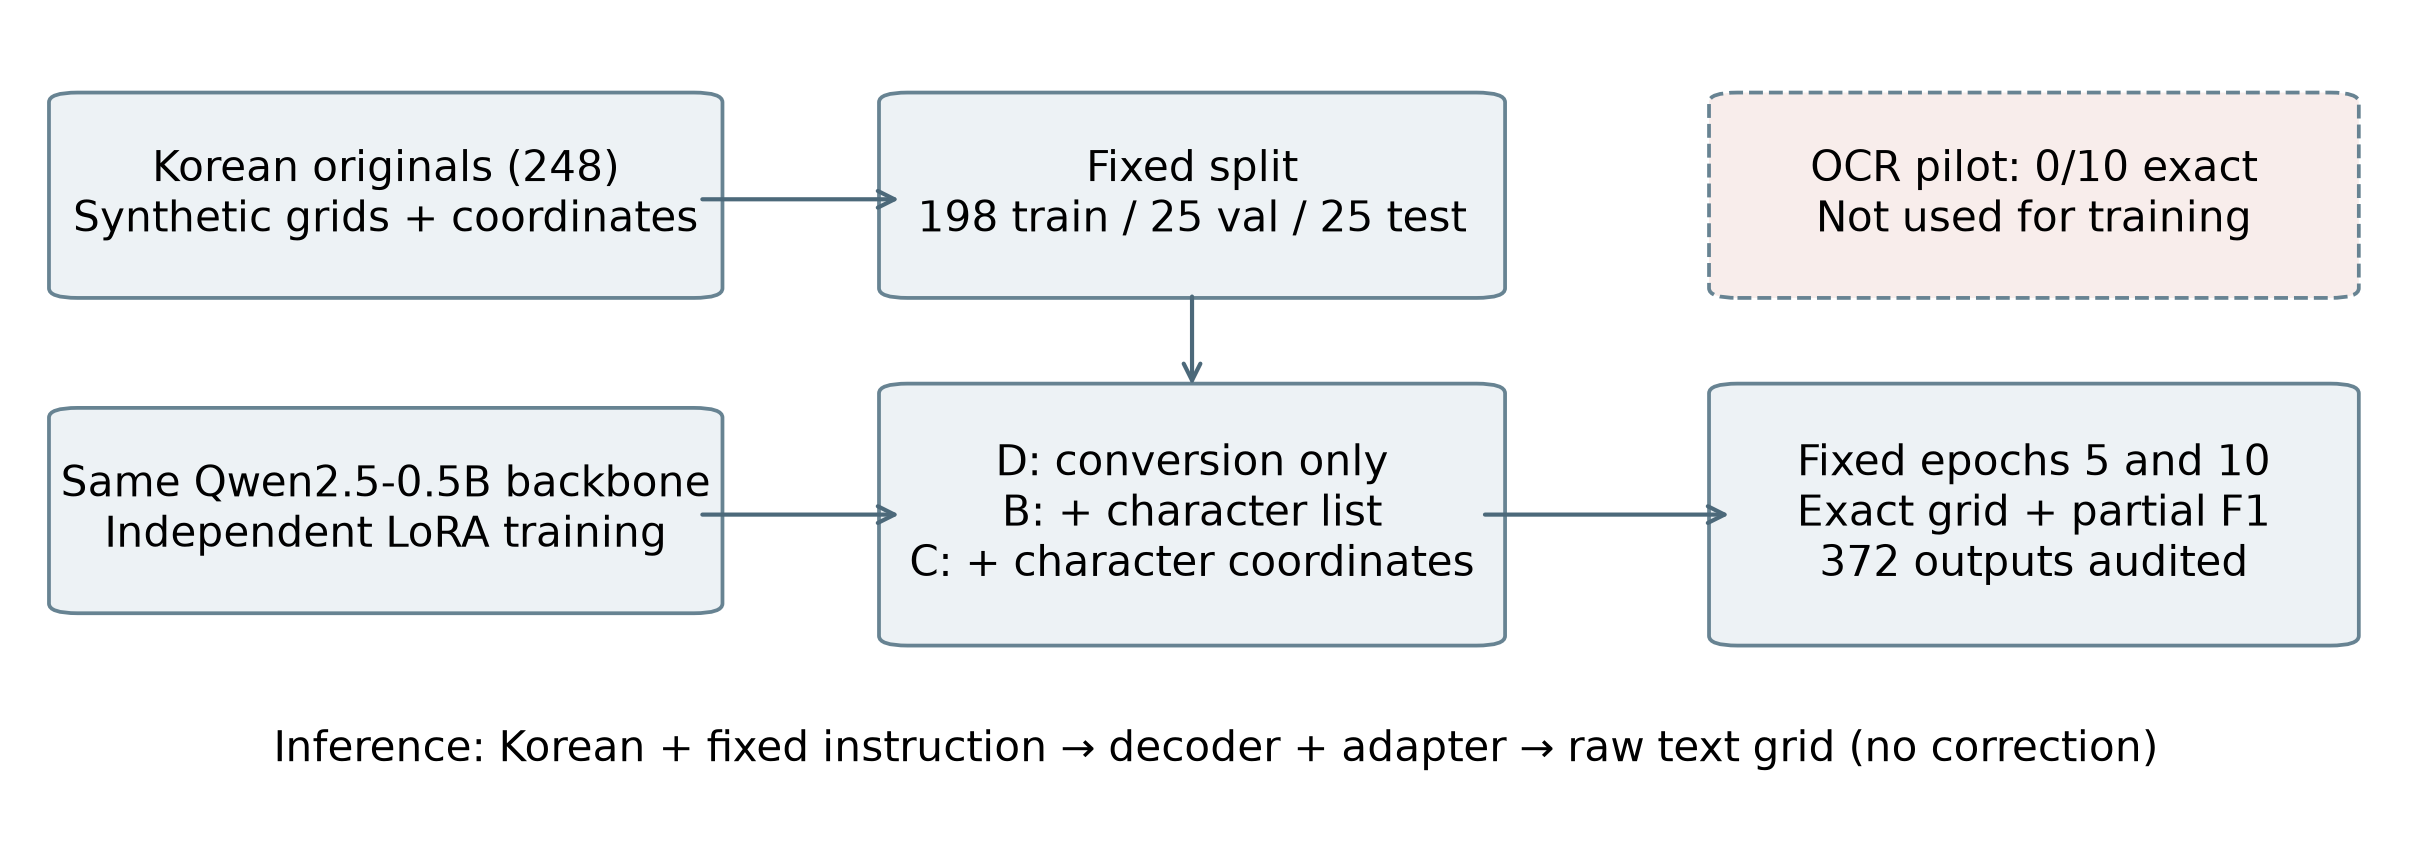
\includegraphics[width=.94\textwidth]{figures/architecture_en.png}
\caption{Training and evaluation architecture. Synthetic annotations supervise D/B/C, which share a backbone specification but have independently trained adapters. Inference generates the grid directly. The deterministic annotation program never repairs predictions. OCR remains a separate failed feasibility pilot.}
\label{fig:architecture}
\end{figure*}

\subsection{OCR feasibility and protocol history}
An initial EasyOCR pilot used ten rendered examples with Korean and English recognition enabled. Raw detections, confidence scores, and bounding boxes were preserved. No image achieved an exact character inventory and two produced no detections. We therefore used synthetic labels for the learning comparison. This finding applies to the tested images and pipeline and does not establish a general failure of Korean OCR. More importantly, our subsequent experiment cannot support a claim about the benefit of OCR-derived supervision.

The original experiment trained B/C for five epochs and selected a checkpoint using validation exact-grid count, then inventory-exact count, then the earlier epoch. Every checkpoint tied at zero on both criteria, selecting epoch one in each condition. Original A/B/C test exact-grid scores were all 0/25. After inspecting those failures, the extension added D and partial diagnostics and fixed epoch ten as primary and epoch five as secondary. The same test set was reused. It is therefore not an untouched confirmatory evaluation.

The extension evaluates each of three conditions at two fixed checkpoints on 12 training-diagnostic, 25 validation, and 25 test inputs: 372 generated outputs in 18 files. We reuse the original A outputs under the same model revision, prompt, split, and decoding configuration. No checkpoint is selected using extension test scores. All inference uses the fixed English conversion instruction, greedy decoding, and at most 256 new tokens. We do not vary prompt language or evaluate few-shot prompting.

\subsection{Metrics and analysis}
Exact grid accuracy is the fraction of full predictions matching $G(x)$ after converting CRLF to LF, removing trailing ASCII spaces on each row, and trimming exterior newlines. Interior whitespace, explanations, and code fences are retained. Inventory-exact accuracy compares multisets of non-whitespace characters. These strict measures indicate whole-output success.

For partial diagnostics, let $P_i$ and $T_i$ be predicted and reference non-whitespace character multisets, and let $Q_i$ and $R_i$ be their sets of $(c,x,y)$ tuples. Micro inventory and coordinate F1 are
\begin{align}
F_{\mathrm{inv}}&=\frac{2\sum_i|P_i\cap T_i|}{\sum_i(|P_i|+|T_i|)},\\
F_{\mathrm{coord}}&=\frac{2\sum_i|Q_i\cap R_i|}{\sum_i(|Q_i|+|R_i|)}.
\end{align}
Multiset intersection counts repeated characters with multiplicity. Coordinates are assigned directly from the canonical output's rows and columns, without alignment or correction. These diagnostics distinguish character preservation from placement; neither measures semantics or readability. We also count outputs reaching the generation limit without termination and report paired item-level comparisons. Subgroup analyses are descriptive, with overlapping categories. No significance claim is made from this single-seed, 25-item test.

\section{Results}
\subsection{Backbone behavior and fixed epoch-ten comparison}
Table~\ref{tab:primary} gives the main extension results. The unadapted model has 0/25 exact layouts and 0.16\% on both partial F1 measures. Its outputs often depart from the requested representation: 23/25 contain composed Hangul and 8/25 reach the token limit. These observations characterize one small backbone under one prompt, not all Qwen models or commercial LLM services.

\begin{table}[t]
\caption{Fixed epoch-ten test results ($n=25$). A is the reused unadapted baseline. F1 values are percentages; exact-grid entries are counts.}
\label{tab:primary}\centering
\begin{tabular}{@{}crrrr@{}}\toprule
 & Exact grid & Inventory F1 & Coordinate F1 & Truncated \\\midrule
A & 0/25 & 0.16 & 0.16 & 8/25 \\
D & 1/25 & 53.30 & 26.36 & 0/25 \\
B & 0/25 & 55.98 & 22.16 & 0/25 \\
C & 0/25 & 53.91 & 28.41 & 0/25 \\\bottomrule
\end{tabular}
\end{table}

D improves substantially over A on partial matching but solves only one test input, the two-syllable word meaning ``leg/bridge.'' B has the highest inventory F1, exceeding D by 2.68 percentage points, while its coordinate F1 is 4.20 points lower. Thus, the character auxiliary task does not improve all aspects of generation.

C achieves the highest coordinate F1, exceeding B by 6.25 percentage points and D by 2.04 points. Its inventory F1 is 2.06 points below B. Both B and C still have 0/25 exact layouts and 0/25 inventory-exact outputs; D has 1/25 on both exact measures. For paired per-input coordinate F1, C exceeds B on 11 items, ties on seven, and falls below B on seven. This is a descriptive pattern, not evidence of statistically established superiority. Fig.~\ref{fig:ablation} visualizes the trade-off between partial character preservation and placement.

\begin{figure}[t]
\centering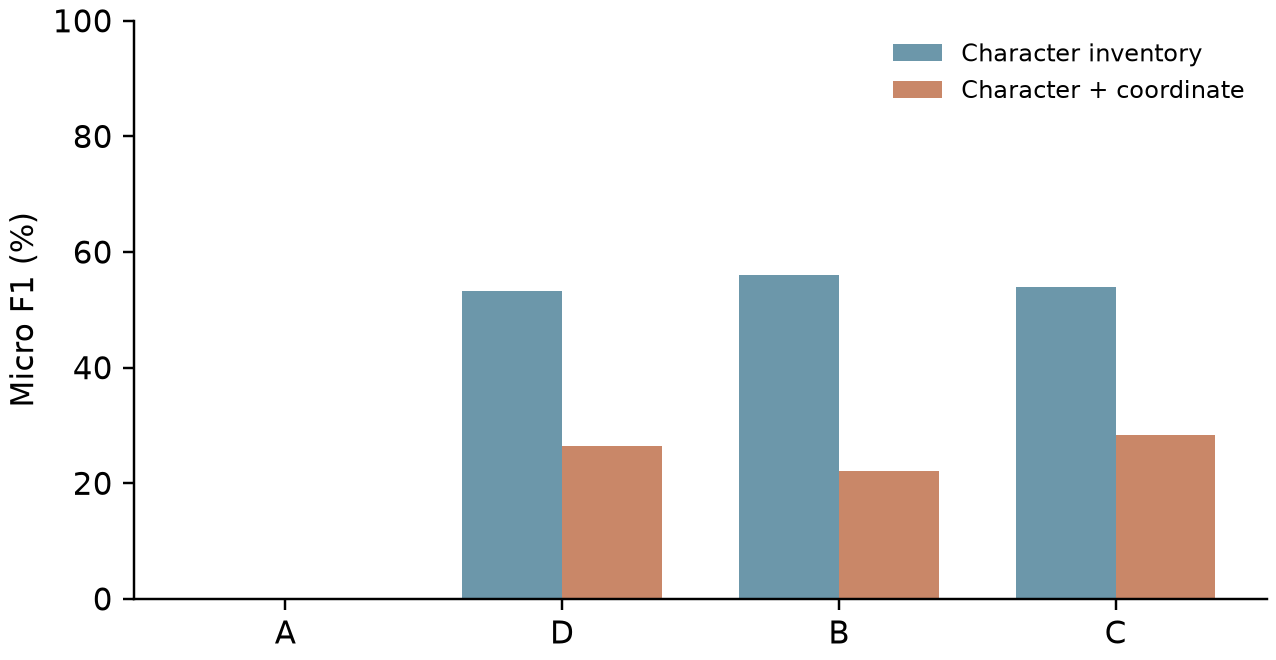
\includegraphics[width=\columnwidth]{figures/ablation_f1.png}
\caption{Epoch-ten component comparison. Both axes of evaluation use micro F1 over all test characters. Higher partial matching does not imply correct complete outputs.}
\label{fig:ablation}
\end{figure}

\subsection{Five versus ten epochs}
Every trained condition improves both partial measures between the two fixed checkpoints (Table~\ref{tab:epochs}). D's coordinate F1 rises from 16.23\% to 26.36\%, B's from 16.87\% to 22.16\%, and C's from 20.00\% to 28.41\%. Only D gains an exact test match. At epoch five, D/B/C have two/one/zero truncated outputs; at epoch ten all have zero. Reduced repetition and improved partial matching therefore coexist with persistent complete-generation failure.

\begin{table}[t]
\caption{Fixed checkpoint comparison on the reused test set. Epoch five here is not the epoch-one model selected in the original experiment. All F1 values are percentages.}
\label{tab:epochs}\centering
\begin{tabular}{@{}ccrrr@{}}\toprule
Condition & Epoch & Exact grid & Inventory F1 & Coordinate F1 \\\midrule
D & 5 & 0/25 & 34.89 & 16.23 \\
D & 10 & 1/25 & 53.30 & 26.36 \\
B & 5 & 0/25 & 40.69 & 16.87 \\
B & 10 & 0/25 & 55.98 & 22.16 \\
C & 5 & 0/25 & 52.57 & 20.00 \\
C & 10 & 0/25 & 53.91 & 28.41 \\\bottomrule
\end{tabular}
\end{table}

\begin{figure*}[t]
\centering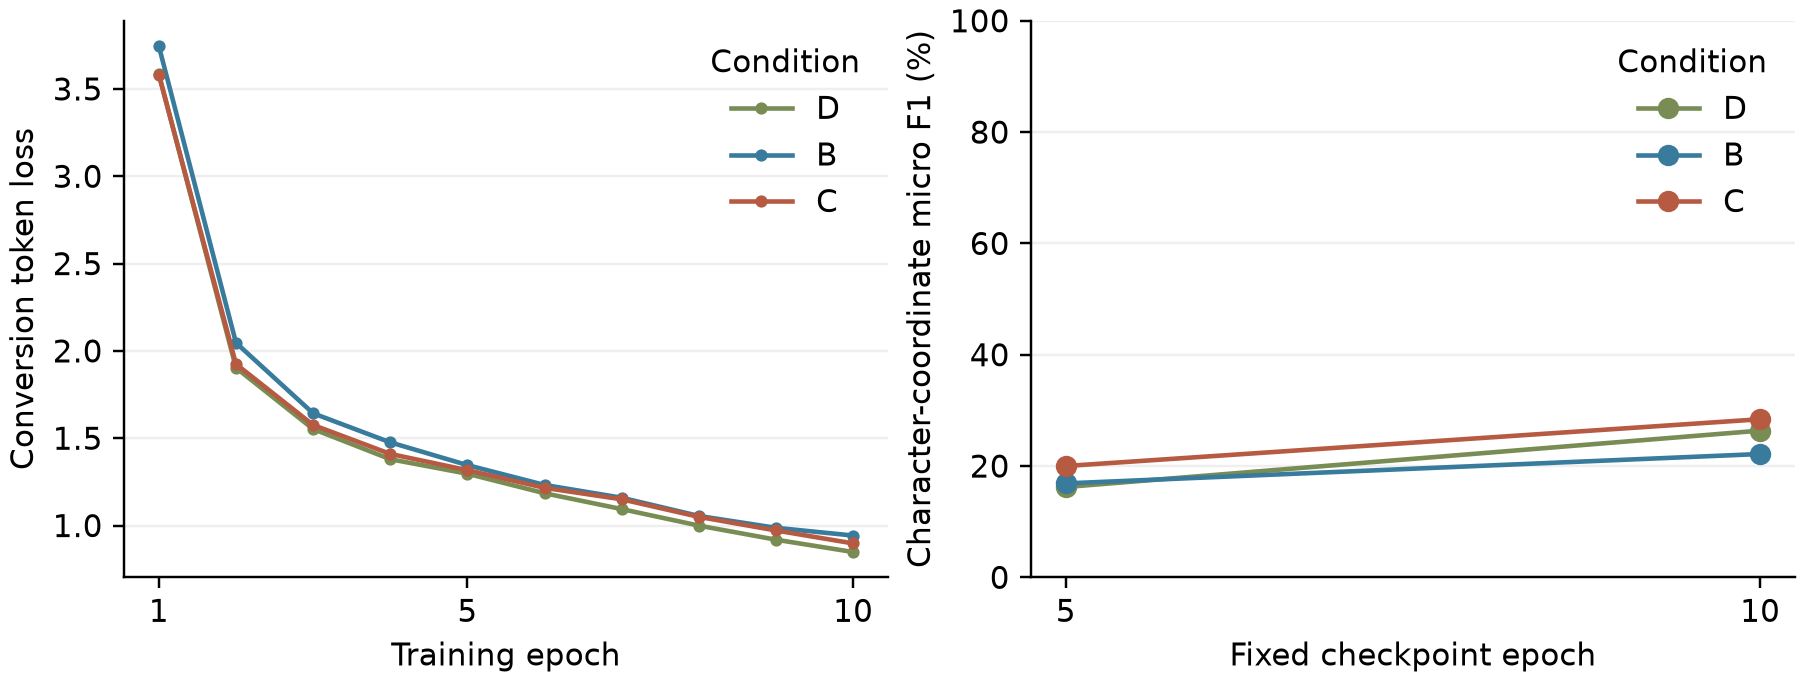
\includegraphics[width=.91\textwidth]{figures/training_and_layout.png}
\caption{Left: conversion loss over ten epochs. Right: fixed-checkpoint test coordinate F1. Loss conditions on reference prefixes; free generation uses the model's own preceding outputs. Neither decreasing loss nor increasing partial F1 establishes exact conversion success.}
\label{fig:learning}
\end{figure*}

\subsection{Training diagnostics and error structure}
At epoch ten, exact generation on the fixed 12-item training subset is 1/12 for D, 0/12 for B, and 1/12 for C. D and C solve the input meaning ``smile.'' Validation exact counts are 0/25, 0/25, and 1/25; C's successful validation item means ``sky.'' Its validation success cannot replace its zero test score. Failures on previously trained inputs make an explanation based solely on generalization to new phrases insufficient. Inadequate fitting, exposure to erroneous generated prefixes, or limited representational capacity remain possible explanations, not isolated causes.

Fig.~\ref{fig:error} illustrates a common error for the input meaning ``giraffe.'' All three epoch-ten conditions replace the first vowel with a different vowel on a lower row and misplace the final consonant. This is not merely a strict-whitespace penalty. The example explains the error type; the aggregate results use all 25 items.

\begin{figure}[t]
\centering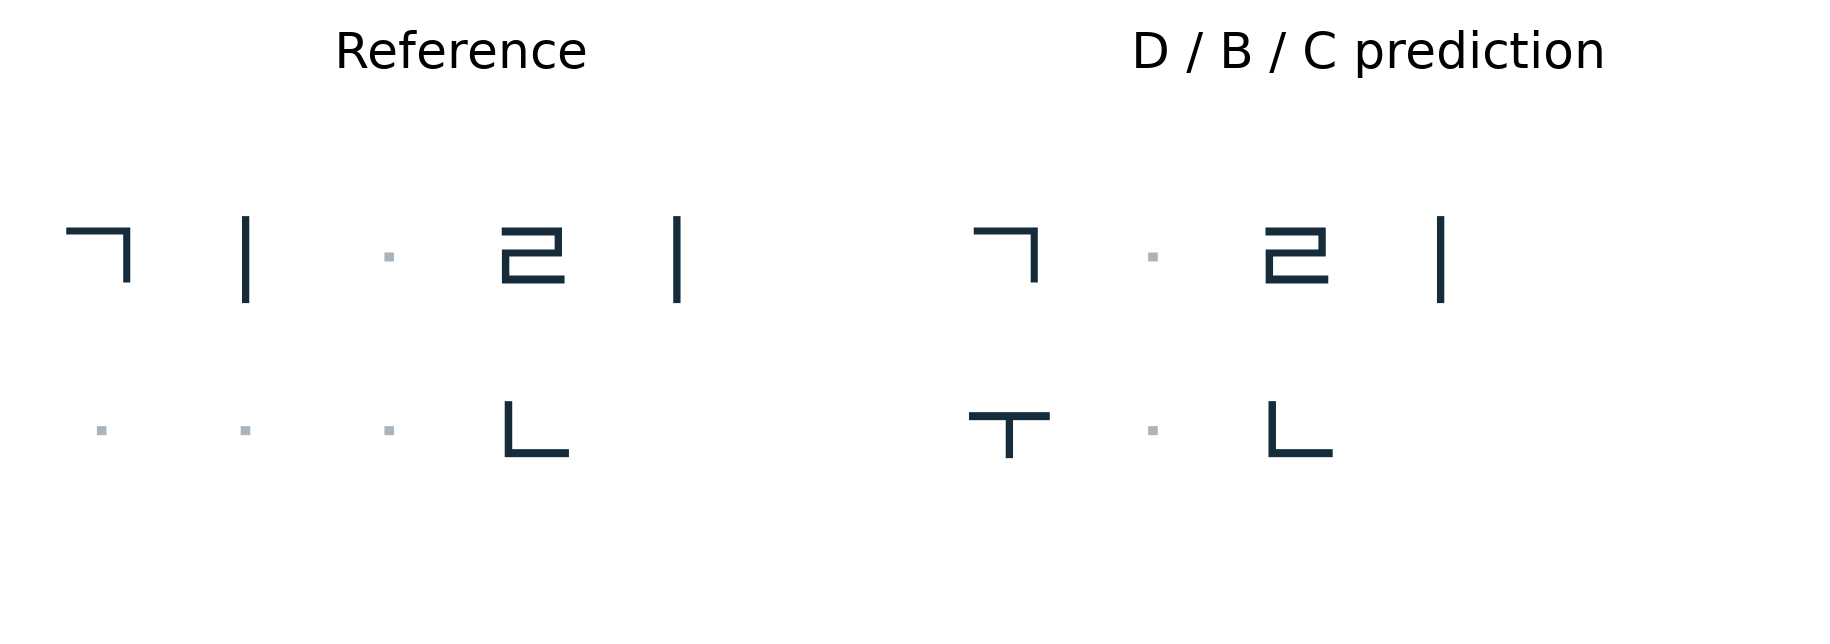
\includegraphics[width=\columnwidth]{figures/error_epoch10.png}
\caption{Full raw epoch-ten outputs for test item ``giraffe.'' D, B, and C produce the same incorrect grid. Dots mark empty cells for inspection only and are not part of the scored strings.}
\label{fig:error}
\end{figure}

Structural groups show uneven differences. For ten inputs without horizontal vowels, B/C coordinate F1 is 16.95/34.78\%; for 15 with horizontal vowels, it is 24.89/25.22\%. For 18 inputs containing final consonants, it is 17.39/25.09\%; for four multiword inputs, 14.16/18.97\%. Length, vowel orientation, and spacing overlap, so these comparisons do not isolate structural causes. The four longest (five-or-more-syllable) inputs are the same four multiword items and must not be treated as independent corroborating groups.

\subsection{Computation and result audit}
Final conversion losses are 0.848, 0.943, and 0.898 for D/B/C. Training-loop times are approximately 5.8, 11.5, and 12.9 minutes, excluding loading and evaluation. Per-epoch target token counts are 2,749, 5,457, and 11,021, excluding prompt tokens. The extension finishes in 39.3 minutes overall. Equal original counts, epochs, and optimizer updates do not match total token exposure or compute. D also assigns a larger weight to conversion loss than B/C. These are important limitations of the component comparison.

All 372 outputs were checked against input IDs, targets, split membership, model paths, and provenance records. Local recomputation matched the exported aggregate and subgroup results. B/C epoch-five validation predictions matched the original run on all 25 items in each condition. Small numerical loss differences and nonidentical adapter files remain, so this does not establish bitwise training reproducibility.

\section{Discussion and Limitations}
\subsection{What the hypotheses support}
H1 receives descriptive support for task adherence and partial matching after adaptation, while exact conversion remains rare. H2 receives mixed support: B preserves more characters than D by inventory F1, but has worse placement and no exact match. For H3, C's partial coordinate score exceeds B's, yet the primary complete-generation criterion does not improve. The defensible conclusion is a limited observation about partial spatial matching, not successful validation of improved exact generation.

The distinction matters for Korean-specific evaluation. Reasoning performance~\cite{naver2025think}, resistance to jamo corruption~\cite{lee2026jamo}, and visual text understanding~\cite{hwang2025kreta} do not automatically establish faithful spatial output. Explicit layout information provides a plausible design direction~\cite{lu2025bounding}, but this experiment does not show that the direction is sufficient. A model may learn pieces of the representation while failing the composition needed for an entire phrase.

\subsection{Limits on causal and external claims}
The dataset is synthetic, small, and restricted to one layout and a subset of vowels. It retains subword overlap across splits and has no human readability study. Only one model size, seed, prompt language, and decoding procedure are tested. The test set was inspected before the extension was designed; fixed extension checkpoints do not remove this dependence. No population-level or statistically significant superiority claim is warranted.

The ablation also changes auxiliary target length and, for D versus B/C, loss composition. A more causal test would match compute or token budgets and examine alternative loss weights, repeated seeds, and new unseen test items. Such experiments are future work, not results reported here. Additional data or constrained generation might improve performance, but the current measurements cannot rank those remedies. Since reference labels are available from explicit rules, OCR is unnecessary for this fixed benchmark; an OCR-specific claim would require genuinely recognized annotations and a separate comparison.

\subsection{Demonstration and reproducibility}
The temporary Colab/Gradio demonstration is an output viewer, not a validated converter. It loads the original validation-selected B epoch-one adapter, keeps raw output intact, and displays characters in equal-width cells. The extension models have not replaced that adapter. The interface explicitly states its 0/25 exact test result and session-dependent availability. There is no rule-based correction or substitution of reference outputs.

The research repository\footnote{\url{https://github.com/kritik-sowieso/AIFFEL_quest_rs/tree/main/MainQuest/Quest03}} accompanies the manuscript with split files, prompts, training and evaluation code, raw outputs, configuration records, and a Korean explanatory notebook. It distinguishes the original run, extension results, and demonstration checkpoint. These materials support inspection of the reported experiment without interpreting the demo as evidence of improved model quality.

\section{Conclusion}
This exploratory study examines coordinate auxiliary supervision for a fixed spatial Hangul jamo generation task. Fine-tuning and additional epochs improve partial character and position matching. At epoch ten, the coordinate condition exceeds character-list supervision by 6.25 percentage points in coordinate micro F1, but both obtain zero exact test layouts; conversion-only training solves one of 25 inputs. Thus, improved complete generation from coordinate supervision is not demonstrated. The contribution is a reproducible task, an explicit component comparison, and failure analysis separating partial spatial progress from successful conversion. The results motivate better-controlled follow-up studies rather than a claim of reliable Korean spatial writing or OCR-enhanced understanding.

\bibliographystyle{IEEEtran}
\bibliography{references}
\end{document}
